\section{Как устроен функционал ошибки в вариационном автокодировщике? За что отвечает каждое из слагаемых?} % Arina

$\sum\limits^{l}_{i = 1}(\mathbb{E}_{q(z|x_{i})}\text{log} p(x_{i} | z) - \text{KL}(q(z|x) || \mathcal{N}(0,1))) \rightarrow max$ \\ 

$q(z|x)$: q -- это кодировщик (полносвязная или сверточная НС), на вход принимает x (картинку), и выдает z, то есть вектор средних и дисперсий. То есть он выдает распределение представлений при условии, что на вход пришла такая-то картинка. \\ 

$p(z|x)$: p -- это декодировщик. Он принимает на вход скрытый вектор и раскодирует картинку. По сути также представляет собой НС. Декодер выдает нормальное распределение с центром в том, что он раскодировал, плюс $\varepsilon$, то есть некий случайный шум.\\ 

$\mathbb{E}_{q(z|x_{i})}\text{log} p(x_{i} | z)$: взяли распределение на скрытых векторах ('облачко'), из него нагенерили кучу точек. Из каждой этой точки развернули новую картинку ($\tilde x_{1}, \tilde x_{2}, \tilde x_{3}$ и т.д.). Далее оценили, насколько каждая из этих раскодированных картинок похожа на оригинальную. По сути мы тут считаем среднюю ошибку рекострукции. Это слагаемое функционала отвечает за то, что мы хотим, чтобы картинки из распределения были похожи на оригинал (оно называется reconstruction likelihood). \\ 

KL -- это дивергенция Кульбака-Лейблера, мера сходства двух распределений (если KL = 0, то распределения одинаковые). Тут мы просим, чтобы распределение, которым кодируется картинка, было как можно больше похоже на стандартное нормальное. Зачем нам это надо? А затем, что кодировщик очень хочет сделать нам вырожденное распределение, и представить его как точку (то есть сделать распределение с очень узким пиком). Это ведет к переобучению -- тогда декодер заучит, во что нужно развернуть именно эту точку, и картинки не особо будут отличаться между собой. Тогда KL -- это что-то типа регуляризатора в нашем функционале. KL позволяет нам расшакалить распределение, на выходе мы получим что-то с центром в 0, но с дисперсией пошире. Если взять только reconstruction likelihood -- получим пустоты в скрытом вектороном пространстве, все будет описано почти что точками, не понятно будет, во что развернуть какую-то случайно выбранную точку между ними. Если взять только KL -- всякие разные картинки перемешаются между собой, так как они все будут описываться стандартным нормальным распределением. Если вместе -- разные картинки будут друг от друга отстоять, но их распределения будут более размазаны. \\ 

\begin{figure}[H]
	\centering
	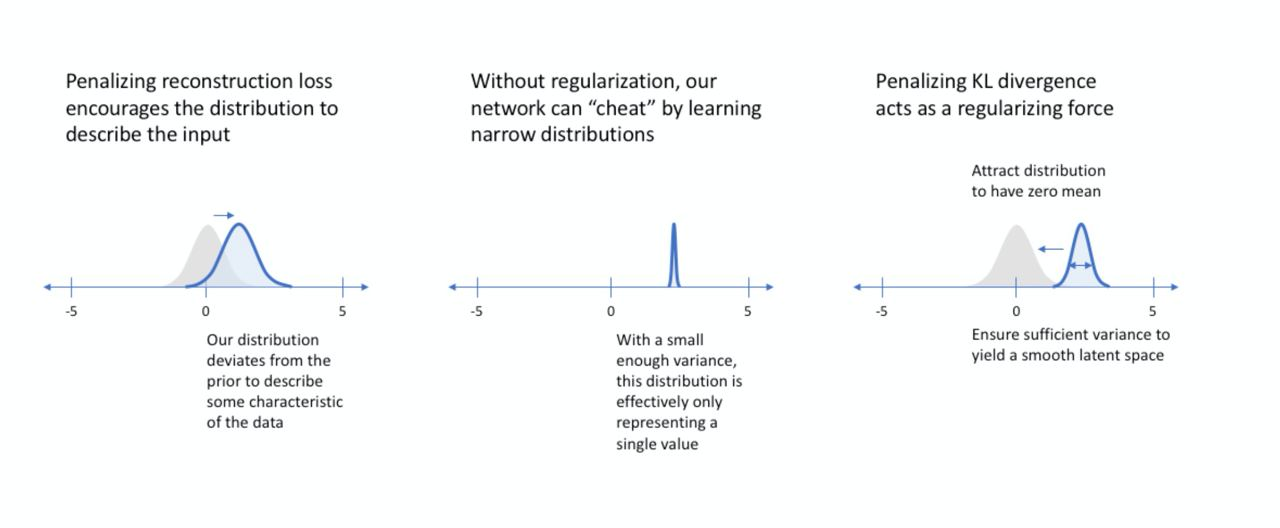
\includegraphics[width=\linewidth]{VAE_loss.jpg}
	\caption{Иллюстрация, что делает KL}
\end{figure}
